\documentclass[First Project.tex]{subfiles}
\begin{document}

\subsection{ Μέθοδος \textlatin{Newton-Raphson} }
Η μέθοδος \textlatin{\textbf{Newton-Raphson}} αποτελεί μία περίπτωση μεθόδου σταθερού σημείου. Προφανώς προϋποθέτει κι αυτή, όπως και η μέθοδος της 
διχοτόμησης, την ύπαρξη ενός διαστήματος \textlatin{\textbf{[a,b]}} στο οποίο η συνάρτηση έχει τουλάχιστον μία ρίζα. Κατ' αναλογία με την μέθοδο της διχοτόμησης
για να βρούμε και πάλι ένα τέτοιο διάστημα χρησιμοποιούμε το θεώρημα \textlatin{\textbf{Bolzano}} σε συνδυασμό με την γραφική παράσταση της 
\textlatin{\textbf{f(x)}}. Εκτός από την ύπαρξη διαστήματος με τις προαναφερόμενες ιδιότητες, η μέθοδος \textlatin{\textbf{Newton-Raphson}} απαιτεί η
εκάστοτε συνάρτηση \textlatin{\textbf{f(x)}} να είναι δύο φορές παραγωγίσιμη σε αυτό το διάστημα με 
\begin{equation*}
    \textbf{\textlatin{$f'(x)$,$f''(x)$}} \neq \textbf{0} \quad \forall \textlatin{x} \in \textlatin{\textbf{[a,b]}}   
\end{equation*}
Καθώς και ένα αρχικό σημείο \textbf{\textlatin{$x_{0}$}} από το οποίο θα ξεκινήσει η επαναληπτική μέθοδος με την εξής ιδιότητα
\begin{equation*}
    \textlatin{f($x_{0}$)} * \textbf{\textlatin{$f''(x_{0})$}} > \textbf{0}
\end{equation*}
\begin{figure}[h!]
    \centering
    \captionsetup{justification=centering}
    \begin{center}
        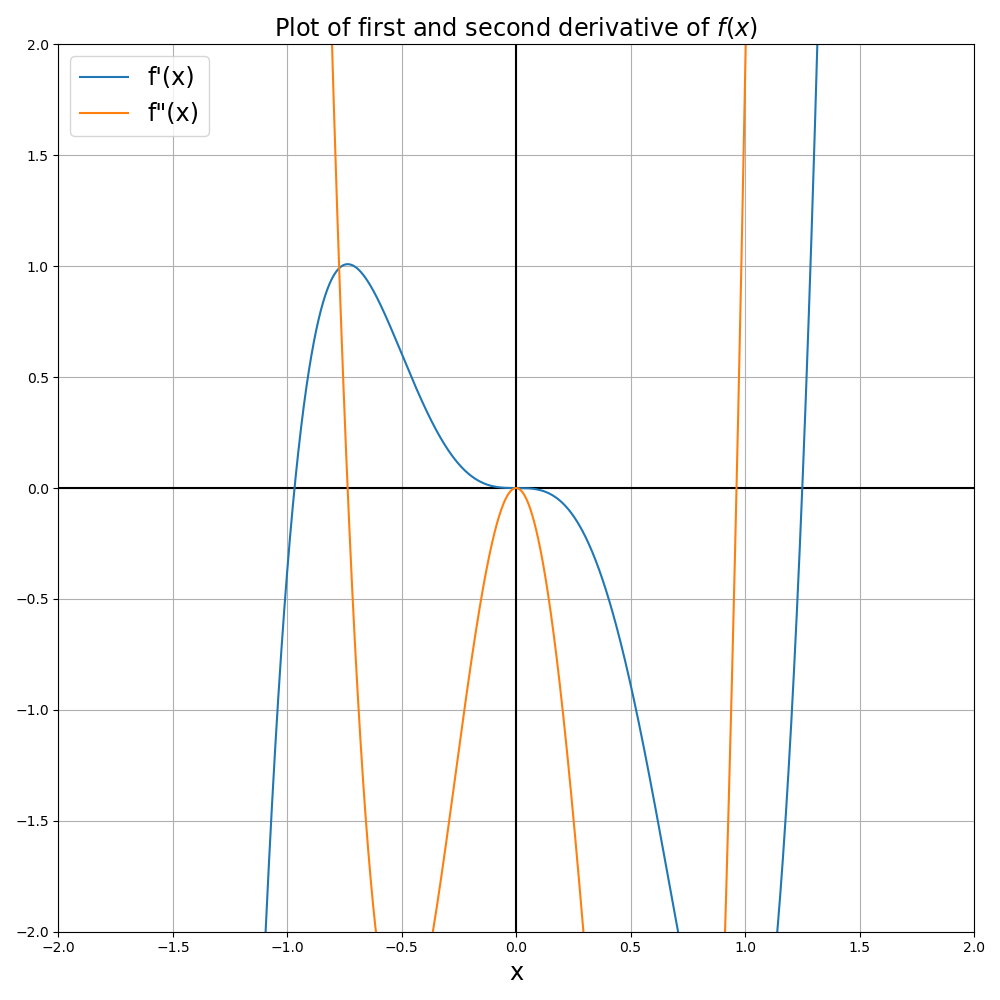
\includegraphics[scale=0.40]{exercise_1_function_derivatives.png}    
        \caption{Γραφική παράσταση της πρώτης και δεύτερης παραγώγου της συνάρτησης \textlatin{\textbf{f(x)}}}
    \end{center}
\end{figure}

Όμοια με πριν παρατηρούμε στο \textit{Σχήμα 1} ότι η δοσμένη \textlatin{\textbf{f(x)}} έχει μία ρίζα στο διάστημα \textlatin{\textbf{[-1.5,-1.0]}} 
καθώς και ότι ισχύει το θεώρημα \textlatin{\textbf{Bolzano}} σε αυτό το διάστημα. Επίσης, παρατηρούμε στο \textit{Σχήμα 10} ότι ισχύει 
\begin{equation*}
    \textbf{\textlatin{$f'(x)$,$f''(x)$}} \neq \textbf{0} \quad \forall \textlatin{x} \in \textlatin{[-1.5,-1.0]}
\end{equation*}

\newpage
Επομένως αρκεί να βρούμε ένα σημείο \textlatin{\textbf{$x_{0}$}} με
\begin{equation*}
    \textlatin{$x_{0}$} \in \textbf{[-1.5,-1.0]}
\end{equation*}
τέτοιο ώστε να ικανοποιείται η συνθήκη
\begin{equation*}
    \textlatin{f($x_{0}$)} * \textbf{\textlatin{$f''(x_{0})$}} > \textbf{0}
\end{equation*}
 
Ένα τέτοιο σημείο είναι το 
\begin{equation*}
   \textbf{\textlatin{$x_{0}$} = -1.4}
\end{equation*}


Για να βρούμε την ρίζα χρησιμοποιούμε την συνάρτηση \textit{\textlatin{\textbf{newton\_raphson}}} από το αρχείο 
\textit{\textlatin{\textbf{newton\_raphson.py}}} με ορίσματα την συνάρτηση \textlatin{\textbf{f(x)}}, την παράγωγο της 
\textlatin{\textbf{f'(x)}} και το αρχικό σημείο \textlatin{\textbf{$x_{0}$= -1.4}}, το \textlatin{\textbf{default}} όρισμα 
\textlatin{\textbf{eps}} έχει την τιμή που χρειάζεται για ακρίβεια \textbf{5} δεκαδικών ψηφίων ενώ το \textlatin{\textbf{default}} 
όρισμα \textlatin{\textbf{max\_iterations}} αντιστοιχεί στον μέγιστο αριθμό επαναλήψεων που θα γίνουν σε περίπτωση που έχει δοθεί κάποιο 
αρχικό σημείο \textbf{\textlatin{$x_{0}$}} χωρίς να τηρούνται οι προϋποθέσεις που εγγυώνται σύγκλιση για την μέθοδο \textlatin{\textbf{Newton-Raphson}}, 
με τιμή τον αριθμό \textbf{50}. Αν πληρούνται όλες οι προϋποθέσεις η συνάρτηση επιστρέφει την ρίζα της \textlatin{\textbf{f(x)}} στο αντίστοιχο
διάστημα \textlatin{\textbf{(a,b)}} ( εδώ στο \textlatin{\textbf{(-1.5,-1.0)}} ), αφού οι προαναφερόμενες προϋποθέσεις εγγυώνται την ύπαρξη 
\textbf{μοναδικής} ρίζας στο διάστημα αυτό, καθώς και τον αριθμό των επαναλήψεων που χρειάστηκαν για να βρέθει η ρίζα με σφάλμα λιγότερο 
από \textlatin{\textbf{eps}}.
\vspace{5px}
\begin{figure}[hp]
    \centering
    \captionsetup{justification=centering}
    \begin{center}
        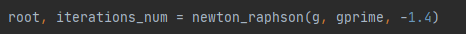
\includegraphics[scale=1]{exercise_1_newton_call_first_root.png}    
        \caption{Παράδειγμα κλήσης της συνάρτησης \textit{\textlatin{\textbf{newton\_raphson}}} με αρχική τιμή \textbf{\textlatin{$x_{0}$ = -1.4}}.}
    \end{center}
\end{figure}


Μετά την κλήση της συνάρτησης \textit{\textlatin{\textbf{newton\_raphson}}} τα αποτελέσματα είναι τα εξής:
\vspace{5px}
\begin{figure}[hp]
    \centering
    \captionsetup{justification=centering}
    \begin{center}
    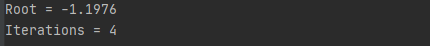
\includegraphics[scale=1]{exercise_1_newton_result_first_root.png}    
    \caption{ Αποτελέσματα κλήσης της συνάρτησης \textit{\textlatin{\textbf{newton\_raphson}}} \\ με αρχική τιμή \textbf{\textlatin{$x_{0}$ = -1.4}}. }
    \end{center}
\end{figure}

Όπου παρατηρούμε ότι η ρίζα της \textlatin{\textbf{f(x)}} στο διάστημα \textlatin{\textbf{[-1.5,-1.0]}} με ακρίβεια 5 δεκαδικών ψηφίων 
είναι η \textbf{-1.1976} καθώς και ότι η μέθοδος \textlatin{\textbf{Newton-Raphson}} χρειάστηκε \textbf{4} επαναλήψεις για να επιτύχει την επιθυμητή ακρίβεια.
Στην συνέχεια παρατηρούμε στο \textit{Σχήμα 1} ότι η \textlatin{\textbf{f(x)}} έχει μία ακόμα ρίζα στο διάστημα \textlatin{\textbf{[1.25,1.75]}} και
πως ισχύει το θέωρημα \textlatin{\textbf{Bolzano}} σε αυτό το διάστημα, όμως δεν ικανοποιείται η πρώτη συνθήκη οπότε θα χρειαστεί να 
περιορίσουμε το διάστημα στο \textlatin{\textbf{[1.3,1.75]}} όπου έχουμε 
\begin{equation*}
    \textbf{\textlatin{$f'(x)$,$f''(x)$}} \neq \textbf{0} \quad \forall \textlatin{x} \in \textlatin{\textbf{[1.3,1.75]}}
\end{equation*}

Επομένως, το επόμενο βήμα είναι η επιλογή του αρχικού σημείου \textbf{\textlatin{$x_{0}$}} έτσι ώστε να ικανοποιείται και η τρίτη συνθήκη.
Ένα τέτοιο σημείο είναι το \textbf{\textlatin{$x_{0}$ = 1.7}}.
Καλούμε λοιπόν την συνάρτηση \textit{\textlatin{\textbf{newton\_raphson}}} με αρχικό σημείο το \textlatin{\textbf{$x_{0}$= 1.7}}.
\vspace{5px}
\begin{figure}[hp]
    \centering
    \captionsetup{justification=centering}
    \begin{center}
        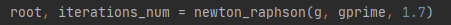
\includegraphics[scale=1]{exercise_1_newton_call_third_root.png}    
        \caption{Παράδειγμα κλήσης της συνάρτησης \textit{\textlatin{\textbf{newton\_raphson}}} με αρχική τιμή \textbf{\textlatin{$x_{0}$ = 1.7}}.}
    \end{center}
\end{figure}


Μετά την κλήση της συνάρτησης \textit{\textlatin{\textbf{newton\_raphson}}} τα αποτελέσματα είναι τα εξής:
\vspace{5px}
\begin{figure}[h!]
    \centering
    \captionsetup{justification=centering}
    \begin{center}
    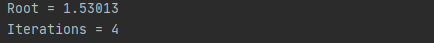
\includegraphics[scale=1]{exercise_1_newton_result_third_root.png}    
    \caption{ Αποτελέσματα κλήσης της συνάρτησης \textit{\textlatin{\textbf{newton\_raphson}}} \\ με αρχική τιμή \textbf{\textlatin{$x_{0}$ = 1.7}}. }
    \end{center}
\end{figure}

Όπου παρατηρούμε ότι η ρίζα της \textlatin{\textbf{f(x)}} στο διάστημα \textlatin{\textbf{[1.3,1.75]}} με ακρίβεια 5 δεκαδικών ψηφίων 
είναι η \textbf{1.5301} καθώς και ότι η μέθοδος \textlatin{\textbf{Newton-Raphson}} χρειάστηκε \textbf{4} επαναλήψεις για να επιτύχει την 
επιθυμητή ακρίβεια. Τέλος, αφού η μέθοδος \textlatin{\textbf{Newton-Raphson}} προϋποθέτει κι αυτή, όπως και η μέθοδος της διχοτόμησης, την 
ύπαρξη διαστήματος στο οποίο ισχύει το θεώρημα \textlatin{\textbf{Bolzano}} για να εγγυάται η σύγκλιση ( εφόσον ισχύουν και οι υπόλοιπες 
προϋποθέσεις ) αντιμετωπίζουμε πάλι πρόβλημα με την ρίζα \textbf{\textlatin{x = 0}}. Αν προσπαθήσουμε να καλέσουμε την συνάρτηση
\textit{\textlatin{\textbf{newton\_raphson}}} με αρχικό σημείο κάποιο σημείο στο οποίο δεν τηρούνται όλες οι προϋποθέσεις τα αποτελέσματα
είναι μη προβλέψιμα και είτε μπορεί να έχουμε σύγκλιση σε λάθος αποτέλεσμα είτε σύγκλιση χωρίς την επιθυμητή ακρίβεια.
\begin{figure}[h!]
    \centering
    \captionsetup{justification=centering}
    \begin{center}
        \begin{tabular}{ |c|c|c| }       
            \hline
            \textbf{\textlatin{$x_{0}$}} & Αποτέλεσμα κλήσης συνάρτησης \textit{\textlatin{\textbf{newton\_raphson}}} & Αριθμός Επαναλήψεων \\
            \hline
            0.25 & 0.00005 & 29 \\ \hline
            0.5 & 0.00009 & 30 \\ \hline
            -0.5 & -0.00005 & 31 \\ \hline
            -0.25 & -0.00004 & 29 \\ [1ex]
            \hline
        \end{tabular}
        \caption{ Αποτέλεσματα κλήσεων της συνάρτησης \textit{\textlatin{\textbf{newton\_raphson}}} χωρίς να τηρούνται όλες οι προϋποθέσεις}
    \end{center}
\end{figure}

Όπως παρατηρούμε και στο σχήμα 15, καμία κλήση δεν βρίσκει την ρίζα της \textlatin{\textbf{f(x)}} με την επιθυμητή ακρίβεια. Η συνάρτηση 
\textit{\textlatin{\textbf{newton\_raphson}}} που έχει υλοποιηθεί στο αρχείο \textit{\textlatin{\textbf{newton\_raphson.py}}} έχει τροποποιηθεί 
έτσι ώστε να ελέγχει αν τo αρχικό σημείο \textbf{\textlatin{$x_{0}$}} αποτελεί ρίζα της \textlatin{\textbf{f(x)}}. Έτσι, αν τώρα
καλέσουμε την συνάρτηση \textit{\textlatin{\textbf{newton\_raphson}}} με αρχικό σημείο το \textlatin{\textbf{$x_{0}$= 0}} και παίρνουμε τα 
εξής αποτελέσματα:
\vspace{5mm}
\begin{figure}[h!]
    \centering
    \captionsetup{justification=centering}
    \begin{center}
    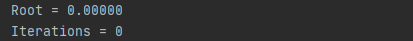
\includegraphics[scale=1]{exercise_1_newton_results_modified_second_root.png}    
    \caption{ Αποτελέσματα κλήσης της τροποποιήμενης συνάρτησης \textit{\textlatin{\textbf{newton\_raphson}}} \\ με αρχικό σημείο \textbf{\textlatin{$x_{0}$ = 0}}. }
    \end{center}
\end{figure}


\newpage

    
\end{document}